\begin{figure*}[ht!]
\begin{minipage}{\linewidth}
\centering
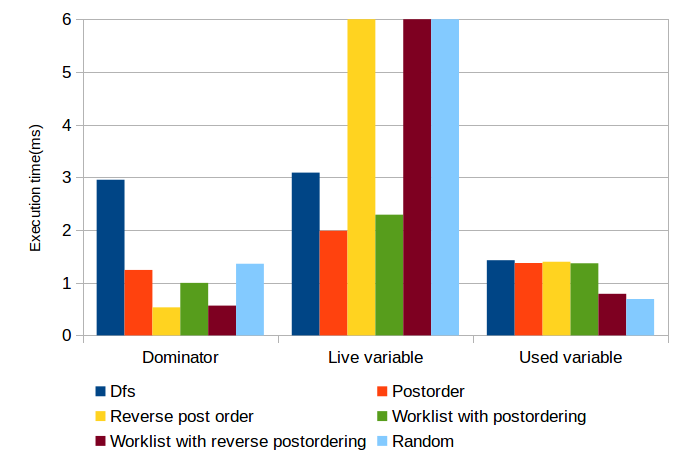
\includegraphics[width=0.74\linewidth]{tex-figures/grapha-motivation.png}
  \caption[Bar chart showing the execution time for dominator analysis, live variable analysis, used variable analysis using dfs traversal, post order, reverse post order traversal, worklist algorithm using post ordering of nodes, worklist algorithm using reverse post ordering of nodes and random order traversal on Graph A. Graph A has 100 nodes and has branches but no loops.]
{Bar chart showing the execution time for dominator analysis, live variable analysis, used variable analysis using dfs traversal, post order, reverse post order traversal, worklist algorithm using post ordering of nodes, worklist algorithm using reverse post ordering of nodes and random order traversal on Graph A. Graph A has 100 nodes and has branches but no loops.}
\label{fig:grapha}
\end{minipage}
\begin{minipage}{\linewidth}
\centering
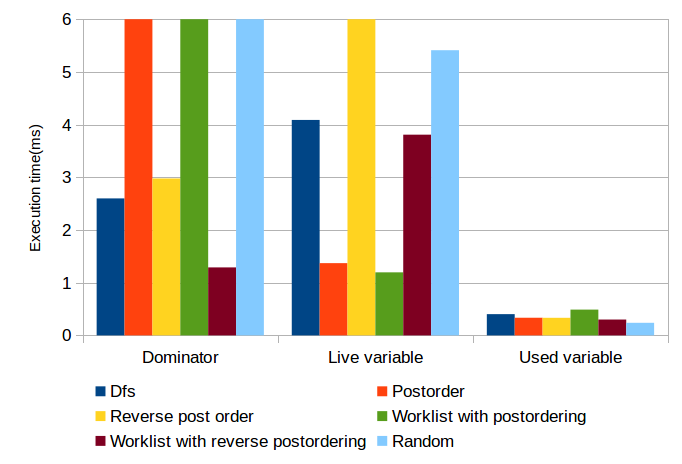
\includegraphics[width=0.74\linewidth]{tex-figures/graphb-motivation.png}
  \caption[Bar chart showing the execution time for dominator analysis, live variable analysis, used variable analysis using dfs traversal, post order, reverse post order traversal, worklist algorithm using post ordering of nodes, worklist algorithm using reverse post ordering of nodes and random order traversal on Graph B. Graph A has 100 nodes and has loops.]
{Bar chart showing the execution time for dominator analysis, live variable analysis, used variable analysis using dfs traversal, post order, reverse post order traversal, worklist algorithm using post ordering of nodes, worklist algorithm using reverse post ordering of nodes and random order traversal on Graph B. Graph A has 100 nodes and has loops.}
\label{fig:graphb}
\end{minipage}

\end{figure*}

